% =============================================================================

\vspace*{\fill}

\begin{figure}[!h]
\begin{lstlisting}[language=pseudo,style=block]
saes.v1.encs rd, rs1 : v1.SubBytes(rd, rs1, fwd=1)
saes.v1.decs rd, rs1 : v1.SubBytes(rd, rs1, fwd=0)
saes.v1.encm rd, rs1 : v1.MixColumn(rd, rs1, fwd=1)
saes.v1.decm rd, rs1 : v1.MixColumn(rd, rs1, fwd=0)
\end{lstlisting}
\caption{
  Instruction mnemonics, and their mapping onto pseudo-code functions, for \ISE{1}.
}
\label{fig:v1:mnemonics}
\end{figure}

\begin{figure}[!h]
\begin{lstlisting}[language=pseudo,style=block]
v1.SubByte(rd, rs1, fwd):
    rd.8[i] = AESSBox[rs1.8[i]] if fwd else AESInbSBox[rs1.8[i]] for i=0..3

v1.MixColumn(rd, rs1, fwd)
    for i=0..3:
        tmp.32  = ROTL32(rs1.32, 8*i)
        rd.8[i] = AESMixColumn(tmp.32) if fwd else AESInvMixColumn(tmp.32)
\end{lstlisting}
\caption{
  Instruction pseudo-code functions for \ISE{1}.
}
\label{fig:v1:pseudo}
\end{figure}

\begin{figure}[!h]
\begin{lstlisting}[language=pseudo,style=block]
lw           a0,  0(a4)       // Load Round Key
lw           a1,  4(a4)
lw           a2,  8(a4)
lw           a3, 12(a4)
xor          t0, t0, a0       // Add Round Key
xor          t1, t1, a1
xor          t2, t2, a2
xor          t3, t3, a3
saes.v1.encs a0, t0           // SubBytes
saes.v1.encs a1, t1
saes.v1.encs a2, t2
saes.v1.encs a3, t3
// Shift rows omitted - 31 Base ISE shift / or instructions.
saes.v1.encm t0, t0           // MixColumns
saes.v1.encm t1, t1
saes.v1.encm t2, t2
saes.v1.encm t3, t3
\end{lstlisting}
\caption{
  An AES encryption round implemented using \ISE{1}.
}
\label{fig:v1:round}
\end{figure}

\vspace*{\fill}

% -----------------------------------------------------------------------------

\newpage

\vspace*{\fill}

\begin{figure}[!h]
\centering
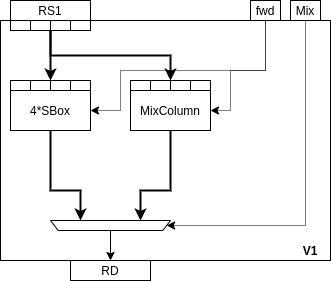
\includegraphics[width={0.5\textwidth}]{diagrams/ise-datapath-v1.png}
\caption{
  A diagrammatic description of the functional unit required to support \ISE{1}.
}
\label{fig:v1:fu}
\end{figure}

\vspace*{\fill}

% =============================================================================
